\section{Results}
This section summarises the results of the project and adds some quantitative
analysis of the implementation. The feature set is fully reflected inside the
implementation section (or the table of contents), so no additional
summarization is done here. Data \emph{file names} refer to the files distributed as \cite*{noauthor_oxrti_data:_2018}.

\subsubsection{Performance}
Currently Cultural Heritage Imaging provides the most frequently used RTI viewer\cite*{noauthor_cultural_nodate-1}. As a result, the performance comparisons have been made with that implementation as the reference. The data is shown
in~\autoref{table_fileformat_results}. The BTF files are about 50\% the size of
the ptm files, and the larger the ptm file, the better the compression benefits are.
The same pattern is evident in the load time as~\autoref{loadtimes} shows. The
bigger the files are, the more profitable the shader implementation, especially
after the one-time conversion is done.
\fig{loadtimes}{Load time comparison}{Orange is the time the RTIViewer takes to
  open the PTM file of the corresponding size. Green is the time oxrti takes to
  convert that PTM file into BTF format. Blue is the time oxrti takes to open
  the corresponding BTF file. Red sums up blue and green. }

\begin{table}[H]
\begin{tabular}{|c | c c c c c c|}
 \hline
 File & Pixel & Conv & Load & Load RTI &
 ptm size & btf size\\
  \hline
  \emph{AK1A\_LRGB} & 3008x2000 & 4906 & 1713 & 11800 & 54.1 & 30  \\
  \emph{Coin\_LRGB} & 7360x4912 & 24674 & 8224 & 59200 & 325.4 & 136  \\
  \emph{Mummy\_RGB} & 583x1000 & 1769 & 627 & 5200 & 10.5 & 5.6  \\
  \emph{tablet2\_LRGB} & 512x512 & 732 & 462 & 1600 & 2.4 & 1.2  \\
  \emph{Warrior\_RGB} & 2299x3200 & 10590 & 2184 & 25500 & 132.4 & 50.2  \\
 \hline
\end{tabular}
\caption[Performance Comparison]{\emph{Pixel} are the dimensions as width x height. \emph{Conv} is the time taken
by the implementation to convert the ptm file to the btf format. \emph{Load} is
the time taken by the oxrti implementation from receiving the btf file to do a complete render. \emph{Load
  RTI} is the approximate time taken by the RTIViewer from opening the file to
finishing the loading. Time was stopped by screenrecording, as no performance
measurements are provided. The time for the processing of mipmaps and normal
maps was excluded, as the oxrti implementation is not doing these steps. The
time to a full first render would be even longer. \emph{ptm size} is the file size in
megabytes. \emph{btf size} is the file size of a plain BTF file (no extra oxrti
state and/or layers). Test runs done on a ``MacBook Pro (Retina, 13-inch, Early
2015); 2.9 GHz Intel Core i5; 16 GB 1867 MHz DDR3; Intel Iris Graphics 6100 1536 MB''. }
\label{table_fileformat_results}
\end{table}

\subsection{Accuracy}
The next thing to verify is the accuracy; it is necessary to determine whether
the implemented rendering is actually giving the 'right' image. To quantify that, the Root Mean Square Error as presented
by Happa and Gogosio\cite*{gogioso_pbr:_2017} was picked, as the RTIViewer
version can be considered the gold standard for this comparison, the pixel dimensions
are equal and all pixel values are calculated with no cross
interactions. The formulae used is:
$$RMSE(X, \overline X )= \sqrt{\frac{\sum_{i=1}^{N} (X_{i}-\overline
    X_{i})}{N}}$$
Where $X$ are the reference pixels, $\overline X$ are the exported pixels, and
$N$ represents the total number of pixels. As each image is an RGB png with
8-bit per channel; this calculation is done for each channel. Pixel values are
in range $[0, 255]$. The images to compare are generated by setting equal light
positions within the LightControl plugin and the RTIViewer and then using the
respective export function. For the oxrti implementation the `fullshot' export
was used, which is exporting after base node rendering in full resolution,
without any further transformation. For the RTIViewer the `Snapshot' button was
used. Due to some bug inside the the RTIViewer implementation some of the
exported images have the wrong dimensions, e.g. the \emph{Mummy\_RGB} is exported
as 583x999 pixels, even though it has 583x1000 pixels. These files were only
compared visually. For \emph{tablet2\_LRGB} and \emph{Warrior\_RGB} the right
dimensions were exported by the RTIViewer. Oxrti exports the right sizes in all
cases. Having one RGB and LRGB file covers all currently implemented  Visuals
comparisons are shown in~\autoref{compare1} and ~\autoref{compare2}, the results
are tabulated in~\autoref{table_Accuracy}. Visual inspection reveals that the
images virtually look the same and the RMSE is confirming this, with less than
one discrete step mean difference between the versions per channel. A
comparison of a completely black with a completely white image would show a RMSE
of 15.96 per channel. The small differences are likely related to shader
architecture. The RTIViewer implementation can operate with pure integers,
whereas the oxrti shaders use floats and their inaccuracies in addition to some
potential texture filtering happening internally.

\begin{figure}
\begin{subfloat}[Warrior from RTIViewer]{\includegraphics[max width=0.32\linewidth]{images/Warrior_RTIViewer}}\end{subfloat}
\begin{subfloat}[Warrior from oxrti]{\includegraphics[max
    width=0.32\linewidth]{images/Warrior_oxrti}}\end{subfloat}
\begin{subfloat}[Mapped diff]{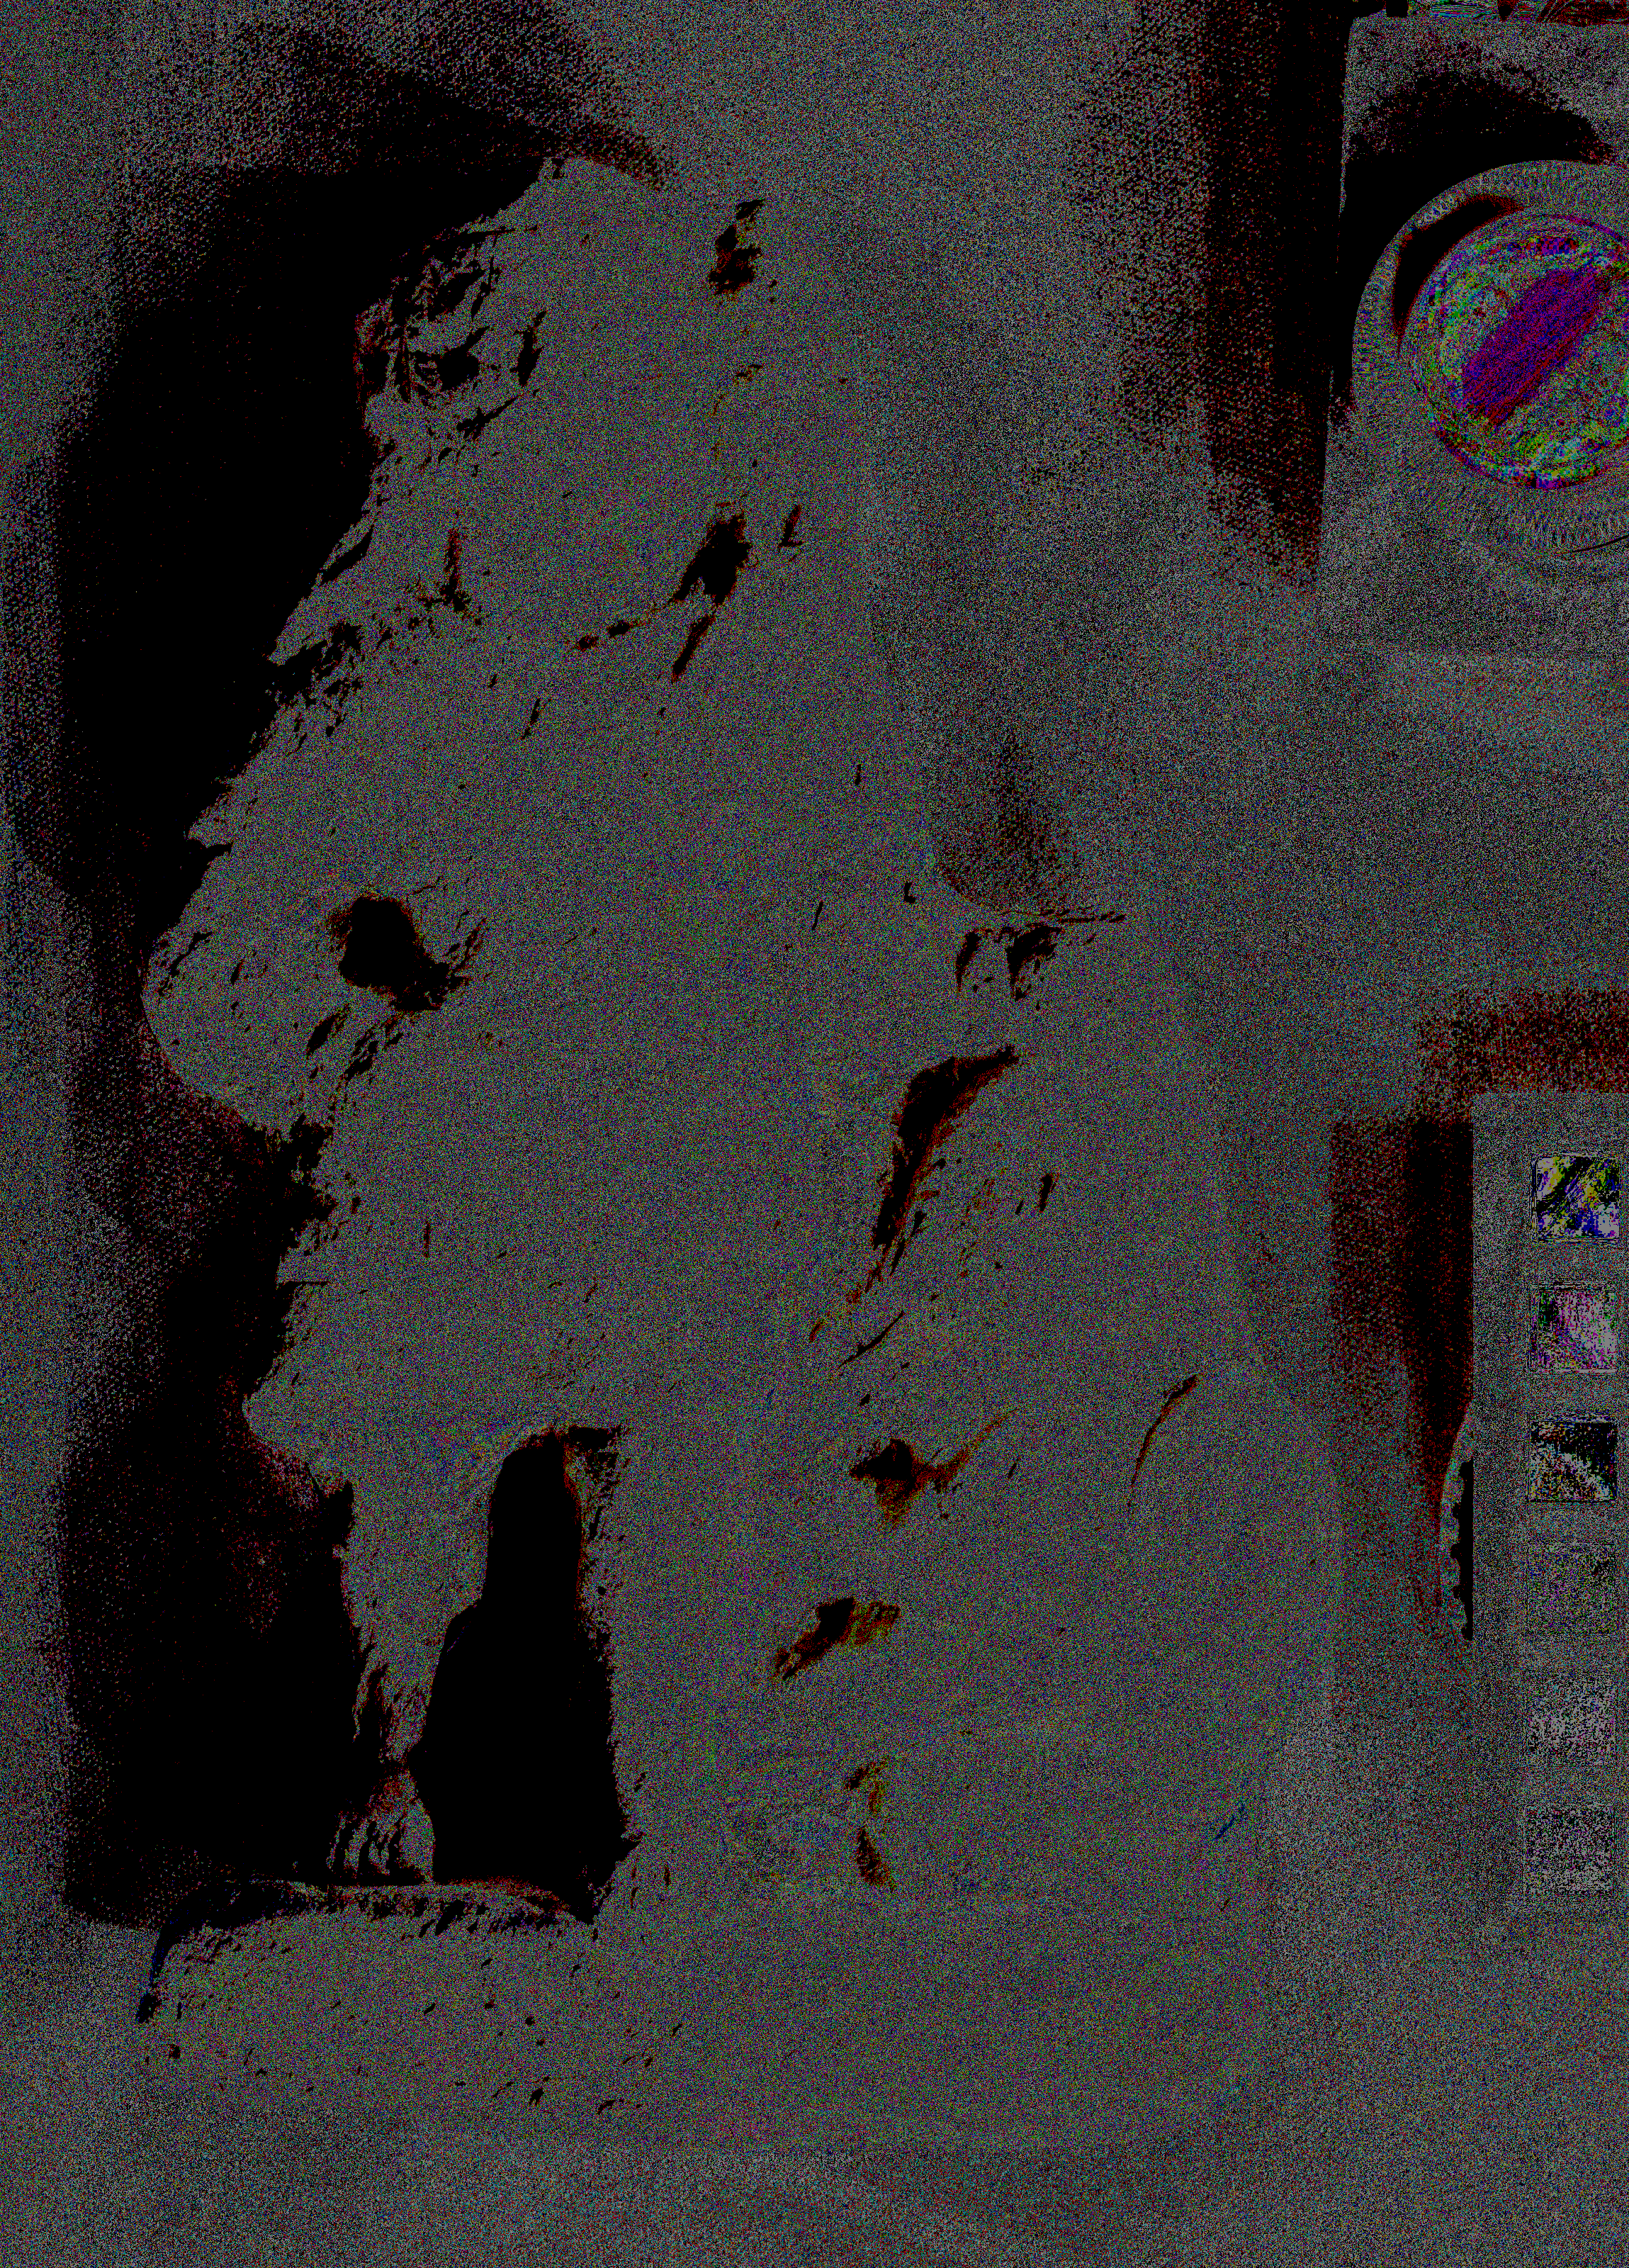
\includegraphics[max width=0.32\linewidth]{images/Warrior_diff}}\end{subfloat}

\caption[Warrior Comparison]{Comparison of RGB rendering between oxrti and RTIViewer. Light position
set in both applications to $x=0.7071, y:=-0.7071$, so a light from bottom
right. The difference is mapped from $[0,1,2]$ to $[0,127,255]$
for visualisation.}
\label{compare1}
\end{figure}

\begin{figure}
\begin{subfloat}[Tablet from RTIViewer]{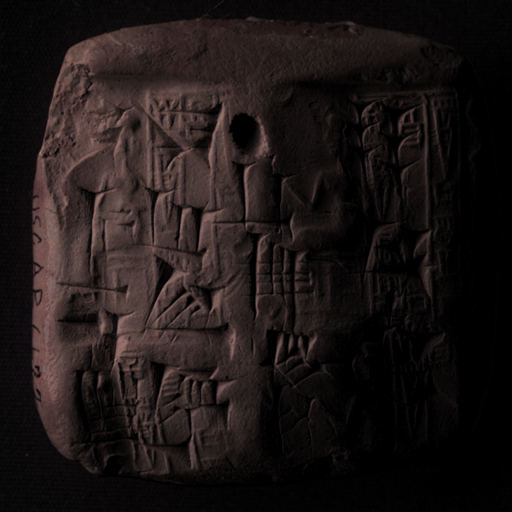
\includegraphics[max width=0.32\linewidth]{images/tablet2_RTIViewer}}\end{subfloat}
\begin{subfloat}[Tablet from oxrti]{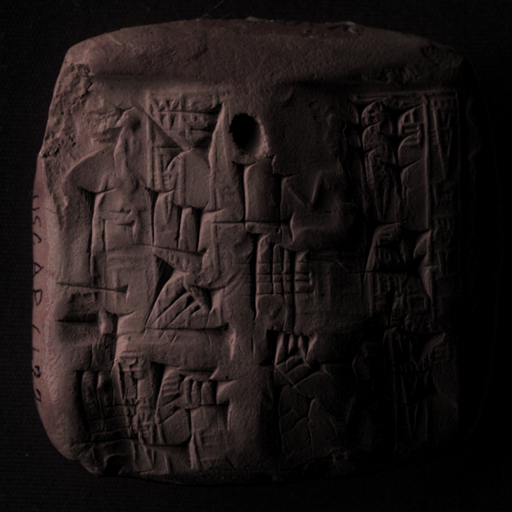
\includegraphics[max
    width=0.32\linewidth]{images/tablet2_oxrti}}\end{subfloat}
\begin{subfloat}[Mapped diff]{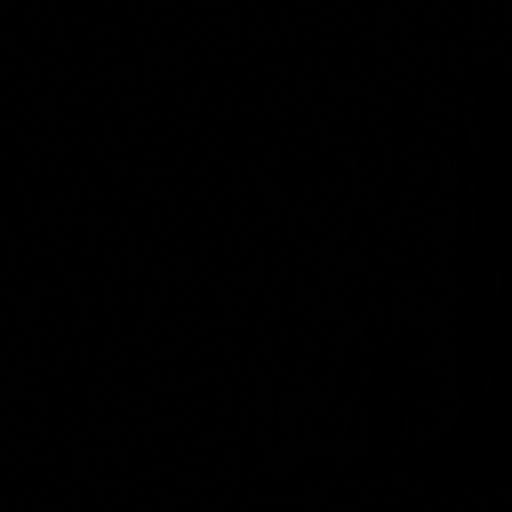
\includegraphics[max width=0.32\linewidth]{images/tablet2_diff}}\end{subfloat}

\caption[Tablet Comparison]{Comparison of LRGB rendering between oxrti and RTIViewer. Light position
set in both applications to $x=-1, y=0$, so a light from the left. The difference is mapped from $[0,1,2]$ to $[0,127,255]$
for visualisation.}
\label{compare2}
\end{figure}

\begin{table}[H]
  \centering
\begin{tabular}{|c |  c c c | c|}
 \hline
 File & RMSE(R) & RMSE(G) & RMSE(B) & SUM  \\
  \hline
  \emph{tablet2\_LRGB} & 0.649 & 0.677 & 0.674  & 2.000 \\
  \emph{Warrior\_RGB} &0.627 & 0.612 & 0.610 & 1.849  \\
 \hline
\end{tabular}
\caption[RMSE for Accuracy Comparison]{RMSE for Accuracy Comparison}
\label{table_Accuracy}
\end{table}

\subsection{Rollouts and Testing}
All versions talked about in~\autoref{sec_apps} are readily available for public
use. Some external testing of these releases has began with participants from the Oxford Centre
for the Study of Ancient Documents (CSAD) and the Institute of Archaeology.
Initial feedback indicates approval of the implementation and will be reported
on in detail at a later point.